\documentclass[aspectratio=43]{beamer}
\usepackage[english]{babel}

\usepackage[thicklines]{cancel}
\usepackage{xcolor}
\usepackage{minted}
\usemintedstyle{emacs}
\usepackage[backend=biber, bibstyle=nature, sorting=nty, citestyle=numeric-comp]{biblatex} %Custom bibliography
    \addbibresource{bib.bib} %Load references

\useoutertheme{infolines}
\useinnertheme{rectangles}
\usefonttheme{professionalfonts}

\definecolor{orange}{HTML}{f28165}
\definecolor{gray}{HTML}{303030}
\definecolor{yellow}{HTML}{f0be52}
\definecolor{lightorange}{HTML}{f19e58}

\renewcommand{\CancelColor}{\color{orange}}

\makeatletter
\newcommand{\mybox}[1]{%
  \setbox0=\hbox{#1}%
  \setlength{\@tempdima}{\dimexpr\wd0+13pt}%
  \begin{tcolorbox}[colback=orange,colframe=orange,boxrule=0.5pt,arc=4pt,
      left=6pt,right=6pt,top=6pt,bottom=6pt,boxsep=0pt,width=\@tempdima]
    \textcolor{white}{#1}
  \end{tcolorbox}
}
\makeatother

\usecolortheme[named=orange]{structure}
\usecolortheme{sidebartab}
\usecolortheme{orchid}
\usecolortheme{whale}
\setbeamercolor{alerted text}{fg=yellow}
\setbeamercolor{block title alerted}{bg=alerted text.fg!90!black}
\setbeamercolor{block title example}{bg=lightorange!60!black}
\setbeamercolor{background canvas}{bg=gray}
\setbeamercolor{normal text}{bg=gray,fg=white}

\setbeamertemplate{footline}
        {
      \leavevmode%
      \hbox{%
      \begin{beamercolorbox}[wd=.333333\paperwidth,ht=2.25ex,dp=1ex,center]{author in head/foot}%
        \usebeamerfont{author in head/foot}\insertshortauthor~~(\insertshortinstitute)
      \end{beamercolorbox}%
      \begin{beamercolorbox}[wd=.333333\paperwidth,ht=2.25ex,dp=1ex,center]{title in head/foot}%
        \usebeamerfont{title in head/foot}\insertshorttitle
      \end{beamercolorbox}%
      \begin{beamercolorbox}[wd=.333333\paperwidth,ht=2.25ex,dp=1ex,center]{date in head/foot}%
        \usebeamerfont{date in head/foot}\insertshortdate{}%\hspace*{2em}

    %#turning the next line into a comment, erases the frame numbers
        %\insertframenumber{} / \inserttotalframenumber\hspace*{2ex} 

      \end{beamercolorbox}}%
      \vskip0pt%
    }

\setbeamertemplate{blocks}[rectangle]
\setbeamercovered{dynamic}

\setbeamertemplate{section page}
{
	\begin{centering}
		\begin{beamercolorbox}[sep=27pt,center]{part title}
			\usebeamerfont{section title}\insertsection\par
			\usebeamerfont{subsection title}\insertsubsection\par
		\end{beamercolorbox}
	\end{centering}
}

\newcommand{\hlight}[1]{\colorbox{violet!50}{#1}}
\newcommand{\hlighta}[1]{\colorbox{red!50}{#1}}
\title{Property Testing With Hedgehog}
\subtitle{Eating Your Bugs}
\author[]{Daniel Cartwright}
\institute[Atlanta Functional Programming]{
    Atlanta Functional Programming
}
\date{August 06, 2019}
\logo{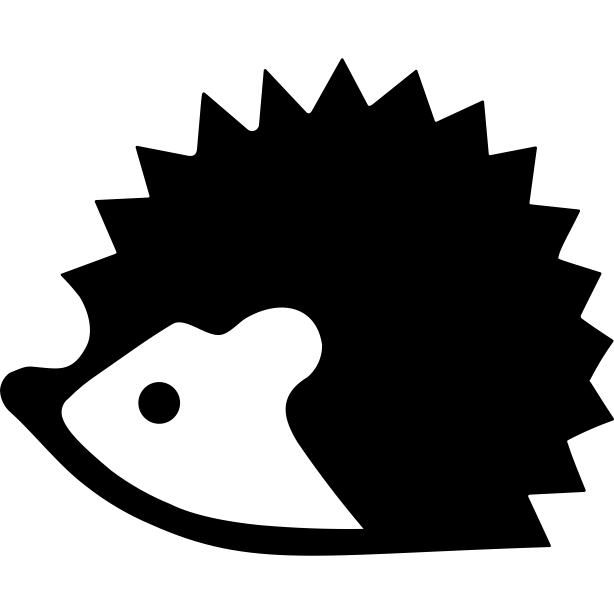
\includegraphics[width= 0.2\textwidth]{images/hedgehog-logo.png}}

\begin{document}
    
    \frame{\titlepage}
    
    \begin{frame}{Summary}
        \tableofcontents
    \end{frame}

    \section{What is Property Testing?}
    
    \frame{\sectionpage}
   
   
    \begin{frame}[fragile]{The Problems With Testing}
        \begin{itemize}
            \item How expensive is breakage?
            \item Tooling (PL, build system, etc.)
            \item Types of testing, verification
            \item Unit Tests are Extremely common
        \end{itemize}
        \begin{minted}[linenos,fontsize=\footnotesize]{haskell}
        -- 'hspec' unit test example
        myAssertion :: Assertion
        myAssertion = myFunction exampleInput `shouldBe` expectedOutput
        \end{minted}
    \end{frame}

   \begin{frame}[fragile]{The Problems With Testing (Cont'd)}
       \begin{definition}{Unit Test}
          A test that checks whether the output of a function, for a single
          example, is equal to the expected output.
       \end{definition}
       
       But, there are problems!
       
       \begin{itemize}
           \item Coverage Problem: Coverage of all code paths
           \item Developer Cost: Costly w.r.t developer time
           \item Unenjoyable to write (bad for morale)
       \end{itemize}
   \end{frame}
   
    \begin{frame}{Property Testing As A Solution To The Coverage Problem}
        Property testing:
            \begin{itemize}
                \item Parametric in its inputs
                \item Based on declarative \textit{properties}, rather than manually-constructed inputs
                \item The inputs are generated, rather than supplied by humans
            \end{itemize}
        
        How do you generate these inputs? Depends:
            \begin{itemize}
                \item Exhaustive property tests
                \item Randomised property tests
                \item Exhaustive, specialised property tests
                \item Randomised, specialised property tests
            \end{itemize}
    \end{frame}

    \begin{frame}[fragile]{Example}
        \begin{minted}[linenos,fontsize=\footnotesize]{haskell}
        prop_reverse :: [Char] -> Bool
        prop_reverse str = reverse (reverse str) == str
        \end{minted}       
    \end{frame}

    \begin{frame}[fragile]{Generators}
        \begin{itemize}
            \item Randomised generators are a way to describe how you should generate some input to a property test
            \item Appropriate generators can be the difference between finding bugs, and not finding bugs
            \item Not all types are easy to generate (e.g.: Word8 vs String)
            \item Generators can often be constructed using combinators, allowing smarter construction of generators (e.g. filtering,sizing)
        \end{itemize} 
        
        Example where a bad generator could fail:
        \begin{minted}[linenos,fontsize=\footnotesize]{haskell}
        prop_isSmall :: [a] -> Bool
        prop_isSmall ls = length ls < 100
        \end{minted}
    \end{frame}
   
    \begin{frame}[fragile]{Shrinking}
        \begin{itemize}
            \item Property test failures result in counterexamples can be large
            \item This can make reasoning about the failure harder
            \item What if we could shrink counterexamples to manageable sizes?
        \end{itemize} 
        
        \begin{minted}[linenos,fontsize=\footnotesize]{haskell}
        prop_allLower :: [Char] -> Bool
        prop_allLower str = all isLower (map toLower str)
        
        -- Counterexample
        -- "As5Enu3au04"
        
        -- Shrunken counterexample
        -- "1"
        
        -- λ toLower '1'
        -- '1'
        \end{minted}
        
        Note that the shrunk counterexample "1" is not necessarily part of the
        original counterexample.
    \end{frame}
    
    \begin{frame}[fragile]{Shrinking With Invariants}
        \begin{itemize}
            \item Shrunk values must have been able to come from the generator that generated the unshrunk value
        \end{itemize}
        
        Consider:
        
        \(\forall n. (n > 6) \Rightarrow (n > 5 \land odd(n)) \)
       
        If shrinking does not obey the invariants of the generator:
        
        \begin{minted}[fontsize=\footnotesize]{haskell}
        -- "Failed: the following number larger than six does not pass the property test: 0" 
        \end{minted}
    \end{frame}



    
    \section{Approaches To Property Testing}

  \frame{\sectionpage}

  \begin{frame}{Libraries}
    \begin{table}
      \begin{center}
        \caption{Property Testing Libraries In Various Languages}
        \begin{tabular}{l|S}
             \textbf{Language} & \textbf{Libraries} \\
             \hline
             \multirow{C}{}{} & theft \\
             \hline
             \multirow{C++}{}{} & CppQuickCheck \\
             \hline
             \multirow{Clojure}{}{} & test.check \\
             \hline
             \multirow{Common Lisp}{}{} & cl-quickcheck \\
             \hline
             \multirow{Coq}{}{} & QuickChick \\
             \hline
             \multirow{Erlang}{}{} & QuickCheck \\
             \hline
             \multirow{F\#}{}{} & FsCheck \\ & Hedgehog \\
             \hline
             \multirow{Golang}{}{} & gopter \\ & quick \\
        \end{tabular}
      \end{center}
    \end{table}
  \end{frame}
  
  \begin{frame}{Libraries (Cont'd)}
    \begin{table}[h!]
      \begin{center}
        \caption{Property Testing Libraries In Various Languages}
        \begin{tabular}{l|S}
             \textbf{Language} & \textbf{Libraries} \\
             \hline
             \multirow{}{}{Haskell} & QuickCheck \\ & Hedgehog \\ & Validity \\ & SmallCheck \\
             \hline
             \multirow{}{}{Java} & QuickTheories \\
             \hline
             \multirow{}{}{Javascript} & jsverify \\
             \hline
             \multirow{}{}{PHP} & Eris \\
             \hline
             \multirow{}{}{Python} & Hypothesis \\
             \hline
             \multirow{}{}{Ruby} & Rantly \\
             \hline
             \multirow{}{}{Rust} & QuickCheck \\
             \hline
             \multirow{}{}{Scala} & ScalaCheck \\
             \hline
             \multirow{}{}{Swift} & SwiftCheck \\
             \hline
        \end{tabular}
      \end{center}
    \end{table}
  \end{frame} 

  \begin{frame}[fragile]{QuickCheck}
      \begin{itemize}
          \item Pioneer of randomised property testing
          \item uses `Arbitrary` typeclass for things that can be generated
          \item uses `Testable` typeclass for things that are testable
      \end{itemize}
      
      \begin{minted}[fontsize=\footnotesize]{haskell}
      class Arbitrary a where
        arbitrary :: Gen a
        shrink :: a -> [a]
      \end{minted}
 
      Example:
      \begin{minted}[fontsize=\footnotesize]{haskell}
      λ> quickCheck $ \(str :: String) -> reverse (reverse str) == str
      \end{minted}
  \end{frame}

  \begin{frame}[fragile]{QuickCheck (Cont'd)}
     \begin{minted}[fontsize=\footnotesize]{haskell}
     reflexive :: Arbitrary a => (a -> a -> Bool) -> Property
     reflexive rel = \x -> x `rel` x 
     \end{minted}
     
     But there's a problem:
     \begin{itemize}
         \item This combinator can only test reflexivity of a given binary relation
               if the relation is reflexive for \textit{all} possible values that
               may be generated by the arbitrary generator.
     \end{itemize}
    
     This is already a problem with `Rational` and `Eq`. The `Eq` instance for `Ratio a`
     assumes that values are normalised:
     
     \begin{minted}[fontsize=\footnotesize]{haskell}
     > 2 :% 2 == 1 :% 1
     False
     \end{minted}
     
  \end{frame}

  \begin{frame}{Problems With QuickCheck}
      `Abitrary` is a lawless typeclass, with no precise semantics!
      
      How should we implement the `Arbitrary` instance for `Rational`?:
      
      \begin{itemize}
          \item Should we ever let it generate 0 :\% 0?
          \item Should we ever let it generate 1 :\% 0?
          \item Should we ever let it generate 5 :\% -1? How about -5 :\% 1?
          \item Should we take the size parameter into account?
      \end{itemize}
      
      There are several considerations:
      
      \begin{itemize}
          \item Never generating un-normalised values could fail to test edge-cases
          \item Generating un-normalised values means we cannot test properties that require (==) to work properly
      \end{itemize}
      
      Solution: newtype wrappers?
      
      But there's a limitation there too...
  \end{frame}

  \begin{frame}{Problems with QuickCheck (Cont'd)}
      \begin{itemize}
          \item Expensive generators and shrinking
          \item QuickCheck docs: "There is no generic arbitrary implementation included because we don't know how to make a high-quality one."
          \item There is no default implementation of `arbitrary`
          \item The default implementation of shrink is `const []`. This means that by default, values are never shrunk!
          \item Developers must implement shrinking themselves, which costs developer time. Moreover, test code is already among the most sloppy, hastily written
          code in most any given codebase.
          \item Orphan instances for `Arbitrary`
      \end{itemize}
  \end{frame}
  
  \begin{frame}[fragile]{Hedgehog}
      \begin{itemize}
          \item Very new approach to property testing (Stanley, J. 2017)
      \end{itemize}
      
      \begin{minted}[fontsize=\footnotesize]{haskell}
      import Hedgehog
      import qualified Hedgehog.Gen as Gen
      import qualified Hedgehog.Range as Range
      
      prop_reverse :: Property
      prop_reverse = property $ do
        xs <- forAll $ Gen.list (Range.linear 0 100) Gen.alpha
        reverse (reverse xs) === xs
      \end{minted}
  \end{frame}
  
  \begin{frame}[fragile]{Hedgehog}
      \begin{itemize}
          \item Free shrinking: Paired with every generator internally
          \item Shrinks are represented as a lazy tree which just needs to be traversed for consecutive shrinks
          \item Much prettier/clearer output, with source
      \end{itemize}
  \end{frame}
  
  \begin{frame}[fragile]{Hedgehog}
      \begin{minted}[fontsize=\footnotesize]{haskell}
      import Hedgehog
      import qualified Hedgehog.Gen as Gen
      import qualified Hedgehog.Range as Range
      import qualified Data.List as List
     
      genIntList :: Gen [Int]
      getIntList =
        let listLength = Range.linear 0 10_000
        in Gen.list listLength Gen.enumBounded
      
      prop_reverse :: Property
      prop_reverse = property $ do
        xs <- forAll genIntList
        reverse (reverse xs) == xs
      
      -- λ> check prop_reverse
      -- ✓ prop_reverse passed 100 tests.
      \end{minted}
  \end{frame}
 
  \begin{frame}[fragile]{Hedgehog}
     Let's do what I do best and write some bad code...
     \begin{minted}[fontsize=\footnotesize]{haskell}
     -- Drops an element somewhere around the middle of the list.
     fauxReverse :: [a] -> [a]
     fauxReverse xs =
       let sx = List.reverse xs
           mp = length xs `div` 2
           (as, bs) = List.splitAt mp sx
       in as <> List.drop 1 bs

     prop_fauxReverse :: Property
     prop_fauxReverse =
       property $ do
         xs <- forAll genIntList
         fauxReverse xs === List.reverse xs
     \end{minted}
  \end{frame}
    
  \begin{frame}[fragile]{Hedgehog}
     And now we test my bad code...
     \begin{center}
     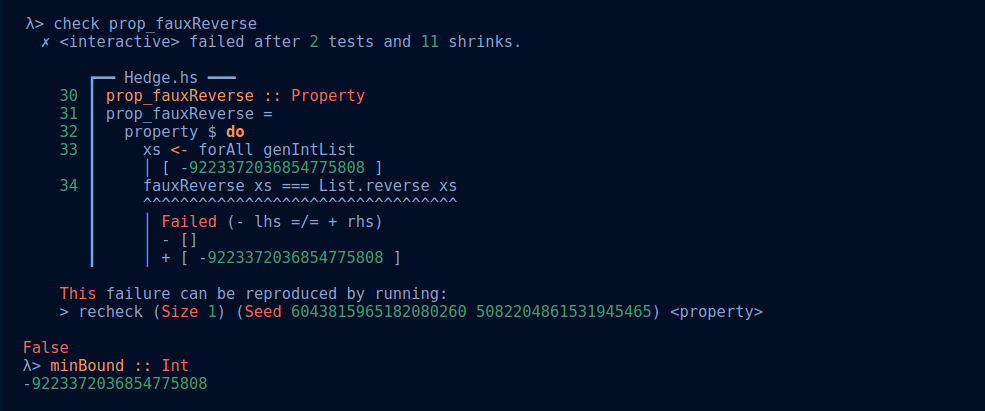
\includegraphics[width= 1.0\textwidth]{images/hedgehog_faux_reverse_output.png}
     \end{center}
  \end{frame}
  
  \begin{frame}[fragile]{Hedgehog}
      \begin{minted}[fontsize=\footnotesize]{haskell}
      -- A reverse function should preserve every element in the list!
      prop_fauxReverseLength :: Property
      prop_fauxReverseLength = property $ do
        xs <- forAll genIntList
        length (fauxReverse xs) === length xs 
      \end{minted}
     
      \begin{center}
      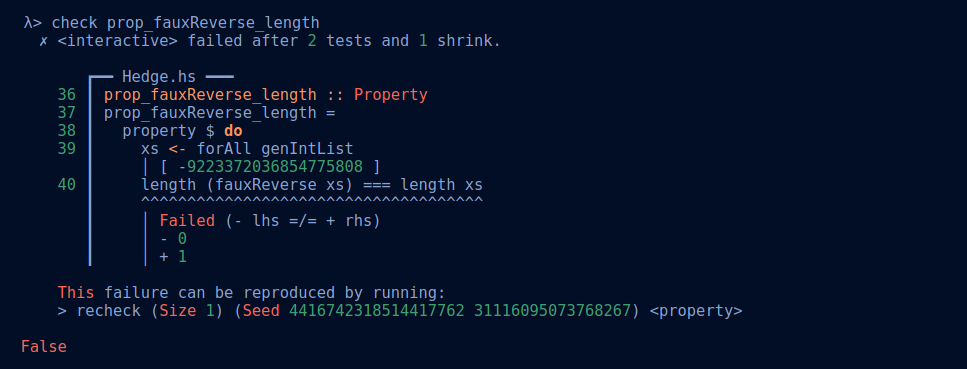
\includegraphics[width= 1.0\textwidth]{images/hedgehog_faux_reverse_length_output.png}
      \end{center} 
  \end{frame}
    
    \section{Real Examples Of Property Testing}

  \frame{\sectionpage}
  
  \begin{frame}{Examples Of Property Testing: Show Me The Code!}
     \begin{center} 
     https://github.com/chessai/hedgehog-talk 
     \end{center}
  \end{frame}
   
    %\section{State Machine Testing}

  \frame{\sectionpage}
  
   
    %\section{Examples of State Machine Testing}

  \frame{\sectionpage}
  
  \begin{frame}{Examples Of State Machine Testing: Show Me The Code!}
     \begin{center} 
     https://github.com/chessai/hedgehog-talk 
     \end{center}
  \end{frame}
    
    \section*{Acknowledgments}
        \begin{frame}{Acknowledgments}
            \begin{itemize}
                \item Thanks to the Atlanta Functional Programming Group for letting me give this talk.
                \item Thanks to Jacob Stanley, Tim Humphries, and the many other Hedgehog contributors
            \end{itemize}
        \end{frame}
    
    \section*{References}
        \begin{frame}{References}
            \nocite{FPComplete} \nocite{Humphries}
            \printbibliography
        \end{frame}

    \begin{frame}{}
        \centering
            \Huge\bfseries
        \textcolor{orange}{Questions?}
    \end{frame}
\end{document}
